\documentclass[10pt]{amsart}
\usepackage{amssymb}
\usepackage{graphics}



\newtheorem{thm}{Theorem}[subsection]
\newtheorem{cor}[thm]{Corollary}
\newtheorem{lem}[thm]{Lemma}

\theoremstyle{remark}
\newtheorem{defn}[thm]{Definition}
\newtheorem*{notation}{Notation}
\newtheorem{alg}[thm]{Algorithm}
\newtheorem{rem}[thm]{Remark}

%opening
\title{Linear Algebra: Answer to Homework 2}
\author{vishvAs vAsuki}

\begin{document}

\maketitle

\section{Question}
Prove that for any $A\in \mathbb{C}^{m\times n}$,
$$ \|A\|_{\infty} = \max_i \|a_i^*\|_1,$$
where $a_i^*$ is the $i$-th row of $A$.
\subsection{Answer}

\begin{notation}
$a_{i,j}$ indicates the element of A at row i and column j. $a_i^*$ is the $i$-th row of $A$. $x_{i}$ and $(Ax)_{i}$ indicates the ith element of vector Ax.
\end{notation}

\begin{thm}
$A\in \mathbb{C}^{m\times n}$,
$$ \|A\|_{\infty} = \max_i \|a_i^*\|_1$$
\end{thm}
\begin{proof}
\begin{eqnarray*}
\|A\|_{\infty} &=& \sup \frac{\|Ax'\|_{\infty}}{\|x'\|_{\infty}}\\
&=& \sup \frac{\|A\alpha x\|_{\infty}}{\|\alpha x\|_{\infty}} , \ with \ \|x\|_{\infty}=1 \texttt{ or } \max(|x_{i}|)=1 \texttt{ constant } \alpha \\
&=& \sup \|Ax\|_{\infty} \\
\end{eqnarray*}

We now see when $\|Ax\|_{\infty}$ is maximum, when $\|x\|_{\infty}=1$.
\begin{eqnarray*}
\|Ax\|_{\infty} &=& \max_{i, x} |(Ax)_{i}| \texttt{ By definiton}\\
&=& \max_{i, x} |a_{i}^{*}x| \\
&=& \max_{i, x} |\sum_{j=1}^{n} a_{i,j}x_{i}| \leq \max_{i, x} \sum_{j=1}^{n} |a_{i,j}x_{i}| \\
&& \texttt{We now maximize with respect to }x_{i}\\
&=& \max_{i, x} \sum_{j=1}^{n} |a_{i,j}||x_{i}| \texttt{ We ensure: }sign(a_{i,j}) = sign(x_{i})\\
&=& \max_{i} \sum_{j=1}^{n} |a_{i,j}| \texttt{ As: }\max(|x_{i}|)=1 \texttt{ We choose: }|x_{i}|=1\\
&=& \max_{i} |a_{i}^{*}|_{1}\\
\end{eqnarray*}
So:
$$ \|A\|_{\infty} = \max_i \|a_i^*\|_1$$
\end{proof}

\section{Question}
Assume $A\in \mathbb{C}^{n\times n}$ and $\exists\ p\geq 1$, s.t. $\|A\|_p < 1$, where $\|.\|_p$ is a vector-induced matrix norm.
\begin{enumerate}
\item Prove that $I-A$ is invertible.
\item Assuming that the series $\sum_{k=0}^{\infty}A^k$ converges, prove that:
$$(I-A)^{-1}=\sum_{k=0}^{\infty}A^k.$$
\item Prove that: 
$$\|A\|_q\|A^{-1}\|_q\geq 1,\ \ \  \forall 1\leq q < \infty.$$
\item Prove that:
$$\frac{1}{1+\|A\|_p}\leq \|(I-A)^{-1}\|_p \leq \frac{1}{1-\|A\|_p}.$$
\end{enumerate}
\subsection{Answer}

\begin{notation}
0 is also used to indicate the 0 vector, whose dimension may be inferred from the context.
\end{notation}

\subsubsection{1.}
\begin{thm}
$I-A$ is invertible.
\end{thm}
\begin{proof}
\begin{eqnarray*}
\|x-Ax \|_{p} + \|Ax\|_{p}&\geq& \|x-Ax +Ax\|_{p} \texttt{:Triangle inequality}\\
\|x-Ax \|_{p} &\geq& \|x\|_{p}  - \|Ax\|_{p}\\
\|(I-A)x \|_{p} &\geq& \|x\|_{p}  - \|Ax\|_{p}\\
\texttt{But, as $\|A\|_p < 1, \forall x$: } \frac{\|Ax\|_p}{\|x\|_{p}} &<& 1\\
\therefore \|(I-A)x \|_{p} &>& \|x\|_{p}  - \|x\|_{p} = 0\\
\end{eqnarray*}
So, I-A does not map any $x \neq 0$ to the 0 vector. So, the null space of I-A consists only of 0.
\end{proof}

\subsubsection{2.}
\begin{thm}
Assuming that the series $\sum_{k=0}^{\infty}A^k$ converges, 
$$(I-A)^{-1}=\sum_{k=0}^{\infty}A^k.$$
\end{thm}
\begin{proof}
\begin{eqnarray*}
(I-A)(I-A)^{-1} &=& (I-A)(\sum_{k=0}^{\infty}A^k)\\
&=& I(\sum_{k=0}^{\infty}A^k) - A(\sum_{k=0}^{\infty}A^k)\\
&=& \sum_{k=0}^{\infty}A^k - \sum_{k=1}^{\infty}A^k\\
&=& A^0 = I\\
\end{eqnarray*} 
\end{proof}

\subsubsection{3.}
\begin{thm}
$$\|A\|_q\|A^{-1}\|_q\geq 1, \ \forall 1\leq q < \infty, \ \forall.$$
\end{thm}
\begin{proof}
It is shown in \cite{trefbau} that: $\|A\|_q\|B\|_q \geq \|AB\|_q$.
So:
$$\|A\|_q\|A^{-1}\|_q \geq \|AA^{-1}\|_q = 1, \ \forall 1\leq q < \infty.$$
\end{proof}

\subsubsection{4.}
\begin{notation}
$\|.\|_{p}$ will be abbreviated to $\|.\|$.
\end{notation}

\begin{lem}
$$\frac{1}{1+\|A\|_p}\leq \|(I-A)^{-1}\|_p .$$
\end{lem}
\begin{proof}
\begin{eqnarray*}
\|(I-A)^{-1} (I-A)\| &\leq& \|(I-A)^{-1} \|\|(I-A)\| \texttt{: By Theorem shown earlier.}\\
1 &\leq& \|(I-A)^{-1} \|\|(I-A)\|\\
\frac{1}{\|(I-A)\|} &\leq& \|(I-A)^{-1} \|\\
\end{eqnarray*} 
But:
\begin{eqnarray*}
\|(I-A)\| &\leq& \|I\| + \|-A\| \texttt{: Triangle inequality}\\
&=& \|I\| + \|A\|\\ 
\frac{1}{\|(I-A)\|} &\geq& \frac{1}{1+\|A\|}\\
\end{eqnarray*}
So, we have the result.
\end{proof}

\begin{lem}
$$\|(I-A)^{-1}\|_p \leq \frac{1}{1-\|A\|_p}.$$
\end{lem}
\begin{proof}

\begin{eqnarray*}
\frac{\|Ax\|_{p}}{\|x\|_{p}} &\leq& \|A\|_{p}\\
\|Ax\|_{p} &\leq& \|A\|_{p}\|x\|_{p}\\
\frac{\|A^{2}x\|_{p}}{\|Ax\|_{p}} &\leq& \|A\|_{p}\\
\|A^{2}x\|_{p} &\leq& \|A\|_{p}\|Ax\|_{p} \leq \|A\|_{p}^{2}\|x\|_{p}\\
\therefore \|A^{k}x\|_{p} &\leq& \|A\|_{p}^{k}\|x\|_{p} \texttt{Provable by induction}\\
\therefore \|A^{k}\|_{p} &\leq& \|A\|_{p}^{k} \\
\|(I-A)^{-1}\| &=& \|\sum_{k=0}^{\infty}A^k\|\\
&\leq& \sum_{k=0}^{\infty}\|A^k\| \texttt{ Triangle inequality}\\
&=& \sum_{k=0}^{\infty}\|A\|_{p}^{k} \\
&=& \frac{1}{1-\|A\|_{p}}\\
\end{eqnarray*}
\end{proof}

From the above lemmata, we have the proof.

\section{Question}
Consider the following procedure to approximate the SVD of a given square matrix $A=U\Sigma V^T$, where $A,U,\Sigma,V \in \Re^{n\times n}$:

\begin{enumerate}
\renewcommand{\labelenumii}{(\roman{enumii})}
\item Initialize $U,\ \Sigma,\ V$ to $I$.
\item Assuming $U,\ \Sigma$ fixed, compute $V$ and orthogonalize it.
\item Assume $U, \ V$ fixed, compute $\Sigma$. Ensure that $\Sigma$ is diagonal and positive.
\item Assuming $\Sigma,\ V$ fixed, compute $U$ and orthogonalize it.
\item If $\|A-U\Sigma V^T\|_F\geq tol$, repeat steps (ii)-(iv).
\end{enumerate}
For simplicity, assume that A is an invertible matrix. 
\begin{enumerate}
\item Implement the above given procedure using Matlab and verify that it converges to the SVD given by Matlab's {\sf svd} command. For verification, run the above given procedure with $tol=1e-5$ for 10 different 50x50 random matrices. Compress all your matlab code in one file and email it to the TA with the subject ``NLA:HW2''. You can use Matlab's {\sf qr} function for orthogonalization. YOU CAN USE MATLAB's STANDARD FUNCTIONS, BUT DO NOT USE ANY CODE FROM THE WEB.
\item Compare the time required by this procedure to that of Matlab's {\sf svd} command. Generate a plot of the time required by your implementation to that of Matlab's {\sf svd} command while varying size of input matrix from 10 to 100. Average your results over 10 different runs. Use matlab's {\sf tic} and {\sf toc} command to measure the elapsed time.
\end{enumerate}

\subsection{Answer}
The code has been emailed to the TA.

\begin{rem}
It turns out that for the procedure to work, a certain way of
calculating V should be used:

   V = inv(A)*U*S; Won't lead to convergence.
   V = (inv(S)*U'*A)'; Gives different V, leads to convergence!

\end{rem}

The graph is shown below (The faster procedure corresponds to the Matlab svd command):

 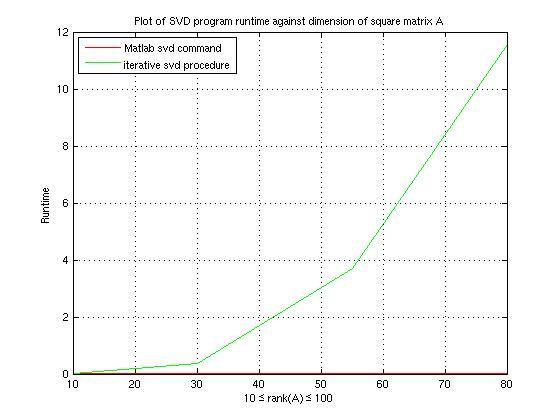
\includegraphics{iterativeSVD.jpg}
 % iterativeSVD.jpg: 0x0 pixel, 0dpi, nanxnan cm, bb=

\bibliographystyle{plain}
\bibliography{../linAlg}


\end{document}
